\documentclass[11pt]{article}

\usepackage[a4paper,margin=3cm]{geometry} % For page dimensions
\usepackage{fontspec} % For font selection
\usepackage{unicode-math} % For mathematical fonts
\usepackage{polyglossia} % For language selection
\usepackage{graphicx} % For images
\usepackage[colorlinks=true, linkcolor=black, urlcolor=blue, citecolor=green]{hyperref} % For hyperlinks
\usepackage{xcolor} % Colors for code highlighting
\usepackage{fancyhdr} % For headers and footers
\usepackage{bookmark}
\usepackage{nameref} % For referencing sections
\usepackage{draftwatermark} % For watermarks
\usepackage{amsmath} % For mathematical equations
\usepackage{listings} % For code formattings
\usepackage{tikz} % For diagrams

\graphicspath{ {images} }

% Set fonts
% \setmainfont{Noto Serif}
\setromanfont{Noto Serif}
\setsansfont{Noto Sans}
\setmonofont{Noto Sans Mono}

% Set languages
\setmainlanguage{greek}
\setotherlanguages{english}

% Header and footer settings
\pagestyle{fancy}
\setlength{\headheight}{14pt}
\fancyhf{}
\fancyfoot[C]{\thepage}

% Custom Commands
\newcommand{\email}[1]{\href{mailto://#1}{\texttt{#1}}} % Email formatting
\newcommand{\developer}[2]{#1 (#2) \\ \email{up#2@ac.upatras.gr} \\[2ex]}
\newcommand{\appname}{Loop}

\author{
    \developer{Γιάννης Ραβασόπουλος}{1100696}
    \developer{Κώστας Λουκανάρης}{1100610}
    \developer{Χρήστος Μάριος Νικολόπουλος}{1100644}
    \developer{Άγγελος Αβεντισιάν}{1100491}
    \developer{Βασίλης Μυλωνάς}{1100643}
}

\date{
    \today \\[1ex]
    Έκδοση 0.1 \\
}


\fancyhead[L]{Περιπτώσεις Χρήσης}
\fancyhead[R]{\leftmark}

\title{
    Περιπτώσεις Χρήσης - \appname\\[1ex]
    \large Τεχνολογία Λογισμικού - ΤΜΗΥΠ, Πανεπιστήμιο Πατρών \\[2ex]
}

\begin{document}

\maketitle
\thispagestyle{empty}
\newpage

\tableofcontents
\newpage

\begin{abstract}
    Περιγραφή των βασικών οντοτήτων και σχέσεων της εφαρμογής \appname,
\end{abstract}

\newpage

\section{Περιγραφή}

\subsection{Find Ride}

Ο χρήστης επιθυμεί να βρεί οδηγό με κοινή διαδρομή με αυτόν για να συμμετέχει σε
κάποια δραστηριότητα (εργασία, μάθημα κλπ).

\subsubsection{Βασική Ροή}
\begin{enumerate}
    \item Ο χρήστης επιλέγει "Find Ride"
    \item Η εφαρμογή εμφανίζει τις δραστηριότητες του χρήστη.
    \item Ο χρήστης επιλέγει μια δραστηριότητα.
    \item To σύστημα εκτελεί αναζήτηση με βάση τα κριτήρια του χρήστη για δραστηριότητες
          άλλων χρηστών που εμφανίζουν τοπική και χρονική ομοιότητα.
    \item Το σύστημα κατατάσει τις δραστηριότητες με βάση την ομοιότητα.
    \item Το σύστημα εμφανίζει τις δραστηριότητες που βρέθηκαν.
    \item Ο χρήστης επιλέγει μια δραστηριότητα.
    \item Το σύστημα εμφανίζει τα στοιχεία του χρήστη που έχει δηλώσει την δραστηριότητα.
    \item Ο χρήστης επιλέγει "Pool".
    \item Το σύστημα ειδοποιεί τον δέκτη και ο χρήστης περιμένει την επιβεβαίωση του.
    \item O δέκτης αποδέχεται την πρόταση του χρήστη.
    \item Το σύστημα ενημερώνει τον χρήστη για τον επιτυχή προγραμματισμό.
\end{enumerate}

\subsubsection{Εναλλακτική Ροή: Ακύρωση 1}

\begin{enumerate}
    \item[3] Ο χρήστης ακυρώνει την αναζήτηση και επιστρέφει στην αρχική οθόνη.
\end{enumerate}

\subsubsection{Εναλλακτική Ροή: Ακύρωση 2}

\begin{enumerate}
    \item[7] Ο χρήστης ακυρώνει την αναζήτηση και επιστρέφει στην αρχική οθόνη.
\end{enumerate}

\subsubsection{Εναλλακτική Ροή: Ακύρωση 3}

\begin{enumerate}
    \item[9] Ο χρήστης αλλάζει γνώμη και πατάει "επιστροφή".
    \item[10] Συνέχεια από το βήμα 6 της βασικής ροής.
\end{enumerate}

\subsubsection{Εναλλακτική Ροή: Απόρριψη Πρότασης}

\begin{enumerate}
    \item[11] Ο δέκτης απορρίπτει την πρόταση του χρήστη.
    \item[12] Συνέχεια από το βήμα 6 της βασικής ροής.
\end{enumerate}

\subsubsection{Εναλλακτική Ροή: Εσωτερικό Σφάλμα}

\begin{enumerate}
    \item[5] Προκύπτει εσωτερικό σφάλμα κατά την αναζήτηση.
    \item[6] Το σύστημα ενημερώνει τον χρήστη για το σφάλμα και προτρέπει τον
        χρήστη σε αναφορά σφάλματος.
\end{enumerate}

\subsubsection{Εναλλακτική Ροή: Ο χρήστης δεν έχει δραστηριότητες}

\begin{enumerate}
    \item[2] Η εφαρμογή προτείνει την δημιουργία μιας δραστηριότητας.
    \item[3] Συνέχεια από το βήμα 1 της βασικής ροής του "Create Activity".
\end{enumerate}

\subsubsection{Εναλλακτική Ροή: Δεν βρέθηκαν όμοιες δραστηριότητες}

\begin{enumerate}
    \item[5] Το σύστημα δεν βρίσκει καμία δραστηριότητα που να ταιριάζει με τα
        κριτήρια του χρήστη.
    \item[6] Το σύστημα ενημερώνει τον χρήστη για την αποτυχία και προτείνει
        τροποποίηση της δραστηριότητας ή τη χρήση δημόσιας συγκοινωνίας.
    \item[7] Ο χρήστης επιλέγει "ΟΚ" και επιστρέφει στην αρχική οθόνη.
\end{enumerate}


\subsection{Create Activity}

Ο χρήστης επιθυμεί να δημιουργήσει μια δραστηριότητα στην εφαρμογή.

\subsubsection{Βασική Ροή}

\begin{enumerate}
    \item Ο χρήστης επιλέγει "Create Activity"
    \item Η εφαρμογή δημιουργεί μια κενή δραστηριότητα και την αποθηκεύει
          προσωρινά.
    \item Συνέχεια από το βήμα 2 της βασικής ροής του use case "Edit Activity".
\end{enumerate}


\subsubsection{Edit Activity}

\begin{enumerate}
    \item Ο χρήστης επιλέγει "Edit Activity".
    \item Η εφαρμογή εμφανίζει μενού με επιλογές για την ιδιότητα του χρήστη (πχ φοιτητής).
    \item Ο χρήστης επιλέγει την ιδιότητα του.
    \item Η εφαρμογή εμφανίζει την φόρμα αναζήτησης και έναν χάρτη της περιοχής του χρήστη.
    \item Ο χρήστης δηλώνει την περιοχή στην οποία επιθυμεί να μετακινηθεί.
    \item Η εφαρμογή εμφανίζει μενού με επιλογές για τις μέρες και τις ώρες έναρξης και λήξης
          της δραστηριότητας.
    \item Ο χρήστης εισάγει τα κατάλληλα στοιχεία.
    \item H εφαρμογή εμφανίζει μενού με επιλόγες για το μέσο μεταφοράς του χρήστη
    \item Ο χρήστης επιλέγει το μέσο μεταφοράς του.
    \item Το σύστημα εκτελεί προεπεξεργασία στα δεδομένα.
    \item Το σύστημα εισάγει την δραστηριότητα στο κατάλογο δραστηριοτήτων του χρήστη.
    \item Η εφαρμογή εμφανίζει μήνυμα επιτυχίας.
\end{enumerate}

\subsubsection{Εναλλακτική Ροή: Ακύρωση 1}

\begin{enumerate}
    \item[3] Ο χρήστης ακυρώνει την διαδικασία και επιστρέφει στην αρχική οθόνη.
\end{enumerate}

\subsubsection{Εναλλακτική Ροή: Ακύρωση 2}

\begin{enumerate}
    \item[5] Ο χρήστης ακυρώνει την διαδικασία και επιστρέφει στην αρχική οθόνη.
\end{enumerate}

\subsubsection{Εναλλακτική Ροή: Ακύρωση 3}

\begin{enumerate}
    \item[7] Ο χρήστης ακυρώνει την διαδικασία και επιστρέφει στην αρχική οθόνη.
\end{enumerate}

\subsubsection{Εναλλακτική Ροή: Ακύρωση 4}

\begin{enumerate}
    \item[9] Ο χρήστης ακυρώνει την διαδικασία και επιστρέφει στην αρχική οθόνη.
\end{enumerate}

\subsubsection{Εναλλακτική Ροή: Μη έγκυρα στοιχεία}

\begin{enumerate}
    \item[7] Ο χρήστης εισάγει μη έγκυρα στοιχεία.
    \item[8] Το σύστημα εμφανίζει μήνυμα σφάλματος και ζητά διόρθωση.
    \item[9] Συνέχεια από το βήμα 6 της βασικής ροής.
\end{enumerate}

\newpage

\subsection{Manage Account}
\label{uc:manage-account}

Ο χρήστης επιθυμεί να ελέγξει ή να ενημερώσει τα στοιχεία του λογαριασμού του.

\subsubsection{Βασική Ροή}

\begin{enumerate}
    \item[1] Ο χρήστης μπαίνει στην ενότητα "Account"
    \item[2] O χρήστης επιλέγει "Profile".
    \item[3] Το σύστημα εμφανίζει τα τρέχοντα προσωπικά στοιχεία.
    \item[4] Ο χρήστης τροποποιεί ένα ή περισσότερα στοιχεία.
    \item[5] Το σύστημα εκτελεί έλεγχο των στοιχείων.
    \item[6] To σύστημα ενημερώνει τα στοιχεία και αποθηκεύει τις αλλαγές.
\end{enumerate}

\subsubsection{Εναλλακτική Ροή: Λανθασμένα Στοιχεία}

\begin{enumerate}
    \item[6] Το σύστημα εμφανίζει μήνυμα σφάλματος και ζητά διόρθωση των στοιχείων.
    \item[7] Ο χρήστης διορθώνει τα στοιχεία.
    \item[8] Συνέχεια από το βήμα 5 της βασικής ροής.
\end{enumerate}

\subsubsection{Εναλλακτική Ροή: Ακύρωση}

\begin{enumerate}
    \item[2] Ο χρήστης επιλέγει το πλήκτρο επιστροφής.
\end{enumerate}

\subsubsection{Εναλλακτική Ροή: Προβολή Ιστορικού}

\begin{enumerate}
    \item[2] Ο χρήστης επιλέγει "History".
    \item[3] Το σύστημα εμφανίζει μια λίστα των συμβάντων \textit{Parking} και
        \textit{Carpooling} στα οποία έχει συμμετάσχει ο χρήστης στο παρελθόν.
    \item[4] Ο χρήστης επιλέγει να δει λεπτομέρειες για κάποιο συμβάν.
    \item[5] Το σύστημα εμφανίζει τις λεπτομέρειες του συμβάντος.
    \item[6] Ο χρήστης επιλέγει το πλήκτρο επιστροφής.
\end{enumerate}

\subsubsection{Εναλλακτική Ροή: Διαγραφή Συμβάντος από το Ιστορικό}

\begin{enumerate}
    \item[2] Ο χρήστης επιλέγει "History".
    \item[3] Το σύστημα εμφανίζει μια λίστα των συμβάντων \textit{Parking} και
        \textit{Carpooling} στα οποία έχει συμμετάσχει ο χρήστης στο παρελθόν.
    \item[4] Ο χρήστης επιλέγει να διαγράψει το συμβάν από το ιστορικό.
    \item[5] Το σύστημα ζητά επιβεβαίωση.
    \item[6] Ο χρήστης επιβεβαιώνει τη διαγραφή.
    \item[7] Το σύστημα διαγράφει το συμβάν από το ιστορικό.
    \item[8] Το σύστημα εμφανίζει μήνυμα επιτυχίας.
\end{enumerate}

\subsubsection{Εναλλακτική Ροή: Προβολή \textit{Rating}}

\begin{enumerate}
    \item[2] Ο χρήστης επιλέγει "Rating".
    \item[3] Το σύστημα εμφανίζει την τρέχουσα βαθμολογία του χρήστη και τυχόν
        σχόλια από άλλους χρήστες.
    \item[4] Ο χρήστης επιλέγει το πλήκτρο επιστροφής.
\end{enumerate}

\newpage

\subsection{Report User}
\label{uc:report-user}

Ο χρήστης επιθυμεί να αναφέρει έναν άλλο χρήστη της εφαρμογής για
παράνομη ή ανεπιθύμητη δραστηριότητα.

\subsubsection{Βασική Ροή}

\begin{enumerate}
    \item Ο χρήστης επιλέγει τον χρήστη που θέλει να αναφέρει και πατάει "Report".
    \item H εφαρμογή εμφανίζει την φόρμα αναφοράς.
    \item Ο χρήστης επιλέγει τον λόγο αναφοράς, προσθέτει σχόλια και επιλέγει "Submit".
    \item Η εφαρμογή ενημερώνει τον χρήστη για την υποβολή.
    \item Το σύστημα επεξεργάζεται την αναφορά και την τοποθετεί σε λίστα αναμονής.
    \item Το σύστημα αναθέτει ποινή στον παραλήπτη της αναφοράς.
\end{enumerate}

\subsubsection{Εναλλακτική Ροή: Απόρριψη Αναφοράς}

\begin{enumerate}
    \item[6] To σύστημα μαρκάρει την αναφορά ως άκυρη και την απορρίπτει.
\end{enumerate}

\subsubsection{Εναλλακτική Ροή: Ακύρωση}

\begin{enumerate}
    \item[3] Ο χρήστης αποφασίζει να μην υποβάλει την αναφορά και πατάει "Cancel".
\end{enumerate}

\newpage

\subsection{Redeem Reward}
\label{uc:redeem-reward}

Ο χρήστης επιθυμεί να λάβει μια ανταμοιβή που έχει κερδίσει μέσω της εφαρμογής.

\subsubsection{Βασική Ροή}

\begin{enumerate}
    \item Ο χρήστης επιλέγει "Redeem Reward"
    \item Η εφαρμογή υπολογίζει τους πόντους του χρήστη.
    \item H εφαρμογή ελέγχει τη διαθεσιμότητα ανταμοιβών.
    \item Η εφαρμογή εμφανίζει τις διαθέσιμες ανταμοιβές και τους πόντους.
    \item Ο χρήστης επιλέγει την ανταμοιβή που επιθυμεί.
    \item Η εφαρμογή ενημερώνει τους πόντους του χρήστη και αφαιρεί την ανταμοιβή
          από τη λίστα των διαθέσιμων ανταμοιβών.
    \item Η εφαρμογή εμφανίζει τον κωδικό εξαργύρωσης.
\end{enumerate}

\subsubsection{Εναλλακτική Ροή: Ακύρωση}

\begin{enumerate}
    \item[5] Ο χρήστης επιλέγει το πλήκτρο επιστροφής.
\end{enumerate}

\subsubsection{Εναλλακτική Ροή: Δεν υπάρχουν διαθέσιμες ανταμοιβές}

\begin{enumerate}
    \item[4] Η εφαρμογή εμφανίζει μήνυμα ότι δεν υπάρχουν διαθέσιμες ανταμοιβές.
\end{enumerate}

\subsubsection{Εναλλακτική Ροή: Ανεπαρκής αριθμός πόντων}

\begin{enumerate}
    \item[6] Η εφαρμογή εμφανίζει μήνυμα ότι ο χρήστης δεν έχει αρκετούς πόντους.
    \item[7] Συνέχεια από το βήμα 4 της βασικής ροής.
\end{enumerate}

\newpage

\subsection{Rate User}
\label{uc:rate-user}

Ο χρήστης επιθυμεί να βαθμολογήσει έναν άλλο χρήστη.

\subsubsection{Βασική Ροή}

\begin{enumerate}
    \item[1] Ο χρήστης επιλέγει "Rate".
    \item[2] Η εφαρμογή εμφανίζει την φόρμα βαθμολόγησης.
    \item[3] Ο χρήστης επιλέγει την βαθμολογία που θεωρεί και προσθέτει σχόλια.
    \item[4] Το σύστημα υπολογίζει τη νέα βαθμολογία του χρήστη και προσθέτει
        την βαθμολόγηση στη λίστα βαθμολογήσεων.
\end{enumerate}

\newpage

\begin{figure}
    \centering
    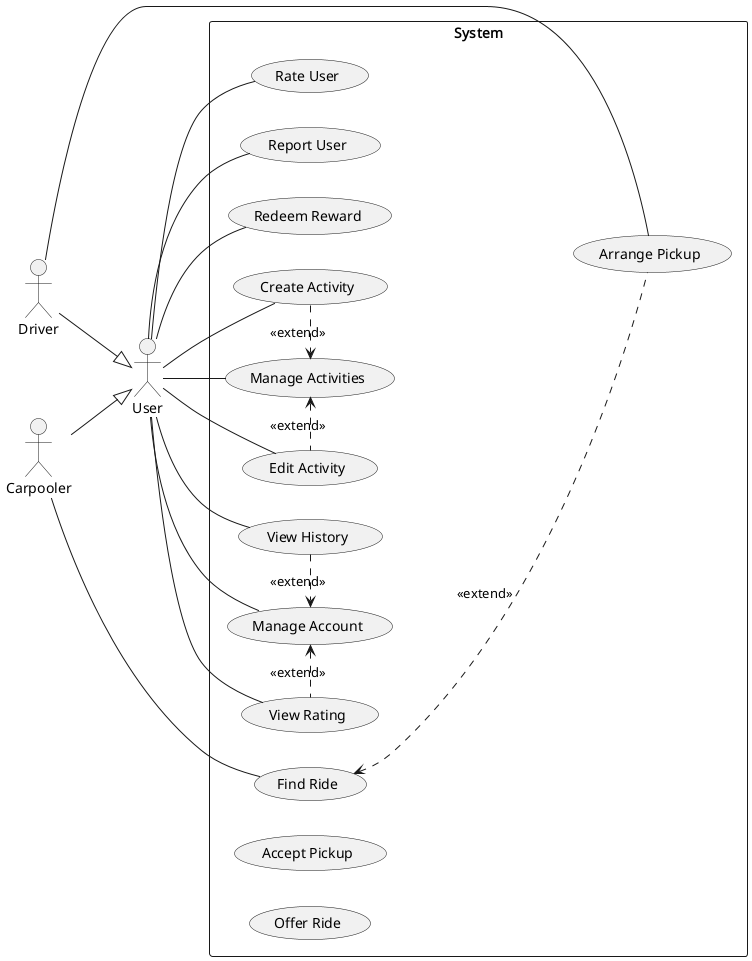
\includegraphics[width=0.8\textwidth]{uml/use-cases}
    \caption{Use Case Diagram}
\end{figure}

\end{document}
